\documentclass[a4paper]{article}

%% Language and font encodings
\usepackage[english]{babel}
\usepackage[utf8x]{inputenc}
\usepackage[T1]{fontenc}

%% Sets page size and margins
\usepackage[a4paper,top=3cm,bottom=2cm,left=3cm,right=3cm,marginparwidth=1.75cm]{geometry}

%% Useful packages
\usepackage{amsmath}
\usepackage{amsfonts}
\usepackage{graphicx}
\usepackage[caption=false]{subfig} % subfigures.  false option prevents conflicts in caption styling with other packages
\usepackage{float}
\usepackage[colorinlistoftodos]{todonotes}
\usepackage[colorlinks=true, allcolors=blue]{hyperref}

%% Custom commands
\newcommand{\DatestampYMD}[3]{\mbox{#1-#2-#3}}
\newcommand{\entry}[3]{\newpage\section*{\DatestampYMD{#1}{#2}{#3}} }

\title{Research Journal}
\author{Stephen Phillips}
\date{June 2018 to Present}

\begin{document}

\maketitle

\entry{2018}{06}{27}
This entry is a bit of catch up, giving some of my initial work and experiments.
\subsection*{Brief High Level Idea}
We are trying to use Graph Neural Networks for feature matching, using cycle consistency as a loss.
What this comes out to in practice is low rank matrix factorization.
However just optimizing typical losses such as the Frobenius norm with a rank loss may not capture real-world noise quite properly.
So the hope is with Neural Nets we can add additional losses to the training for it to incorporate into its factorization at training time, then it will know how to properly do that at testing time.
For now we stick with the aforementioned Frobenius norm to start training.

\subsection*{Literature Review}
\begin{itemize}
\item ``Geometric Deep Learning: Going beyond Euclidean data'' Bronstein et al. 2017.
A survey paper going over many types of non-Euclidean networks.
Here we use the non-fixed structure neural networks.
In particular Kipf and Welling, described below.
\item ``Semi-Supervised Classification with Graph Convolutional Networks'' Kipf and Welling 2017.
This paper takes the graph Laplacian and uses is to multiply a node embedding.
Combine this with weights and non-linearities you have a fully functional neural network.
There was some criticism of this method from \href{https://www.inference.vc/how-powerful-are-graph-convolutions-review-of-kipf-welling-2016-2/}{this blog post} stating that these reduce to rather simple operations when put on a regular graph.
Regardless we will be using this method here.
\item ``The graph neural network model'' Scarselli et al. 2009.
This is a more complicated framework, similar to the previous one but instead using polynomials of the Laplacian instead of just the Laplacian itself.
This gives it more expressively but also means the local nature of it fails to some degree.
This is why I will be using Kipf and Welling as my basis for now.
If that fails, I may try this.
\item ``Relational inductive biases, deep learning, and graph networks'' Battaglia et al. 2018.
This is a high level introduction to a new notion of Graph Neural Networks, with operations on the edges as well as the nodes.
This could be potentially quite helpful but unfortunately there is no implementation of this right now, so using it would be difficult.
For potential future work.
\end{itemize}

\subsection*{Code base}
Initially this was implemented in PyTorch but due to the potential future need for sparse matrices I switched to TensorFlow. The modules of the code are:
\begin{itemize}
\item \texttt{options.py} - This handles all configuration options for building the models, the dataset, and the learning parameters - every other file depends on this one
\item \texttt{model.py} - File with all the models in it - specifically for graph neural networks. All models are sub-classes of \texttt{DenseGraphLayerWeights} which gives a lot of convenience functions for graph networks
\item \texttt{sim\_graphs.py} - Handles synthetic data creation.
\item \texttt{data\_util.py} - Handles generic data creating and loading for graph networks. Has a feature if tensorflow is not able to load it can ignore it and only use Numpy.
\item \texttt{train.py} - Main training file, implements data loading and feeding to neural net pipe-line
\item \texttt{myutils.py} - Lots of convenience functions
\item \texttt{tfutils.py} - Lots of convenience functions but for TensorFlow
\item \texttt{experiment.py} - This is where all the plots are generated. 
\end{itemize}

\subsection*{Exact model}
The input to our neural network is an undirected graph with each node having a starting embedding.
The target is each node having an embedding.
The graph structure is given to us as an $n \times n$ Adjacenty matrix, and the embeddings as an $n \times m$ matrix $E$ (typically $m << n$).
Thus using Kipf and Welling as our guide, we have our update rule for layer $i$ as:
\begin{align*}
D = \mathrm{diag}((A + I) \mathbf{1}) \\
L = D^{-1/2}(A + I)D^{-1/2} \\
E_{i+1} = \sigma \left(LE_{i} W^{(i+1)}\right) + E_{i} U^{(i+1)}
\end{align*}
With $W^{(i+1)}$ and $U^{(i+1)}$ being a $m_i \times m_{i+1}$ matrix, and $E_i$ being a $n \times m_i$ matrix (with $E_0 = E$).
$\sigma$ here is our non-linearity.
The $U$ weights are for skip connections.
The final layer $F$ is each row of the final embedding $E_N$ normalized to norm 1 (here our network has $N$ layers).

This model seems reasonable.
Consider the special case if $m_i = 1$ for all $i$ and $\sigma(x) = x / \|x\|$.
Setting the weights to be 1, we get $E_{i+1} = L E_i / \| L E_i \|$.
This is exactly the power method of finding the leading eigenvectors, which is an approximation of cycle consistency.

\subsection*{Experiments}
First this was generated using 3 random $25 \times 25$ permutation matrices stacked together to form a $75 \times 25$  matrix as the ground truth node embedding vectors $E_{gt}$, then using the outer product to make a $75 \times 75$ matrix $S_{gt} = E_{gt} E_{gt}^\top$, which serves as the ground truth graph.
We have some noise function $\nu$ and so the given graph is $A = \nu(E_{gt})$.
We get our output embedding $F$ So this is essentially testing if we can do matrix factorization via Graph Neural Networks with various noise models.
We have a very noisy initial embedding.
To compute the error, we compute the factored similarity matrix, which means we normalize each embedding row then do an outer product.
For the figures we display the node embedding vectors grouped by the ground truth labels, so the true plots look like a diagonal matrix.

% Figure \ref{fig:baseline_plot} shows an example of ground truth node embedding and similarities as well as the node embedding vectors and similarities of the initial embedding we use.
% 
\begin{figure}[H]
    \centering
    % \includegraphics[width=0.7\textwidth]{figures/noiseless_sim.png}
    \begin{minipage}{.45\linewidth}
        \subfloat[Sorted ground truth embedding and initial embedding]{ 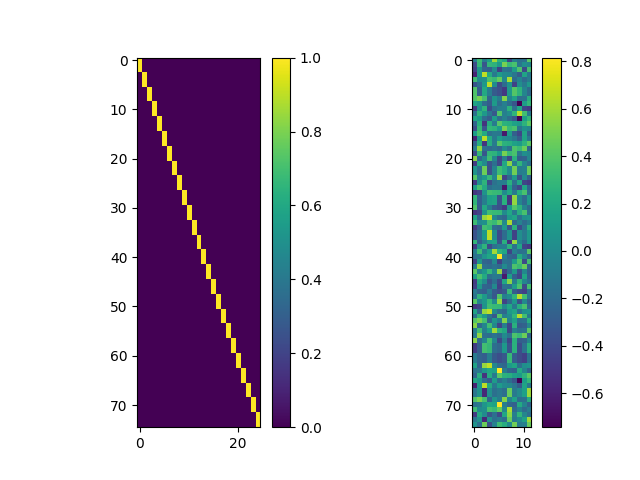
\includegraphics[width=0.9\textwidth]{figures/baseline_embeddings.png} \label{fig:baseline_sub1} }
    \end{minipage}
    \begin{minipage}{.45\linewidth}
        \subfloat[Ground truth and initial similarity]{ 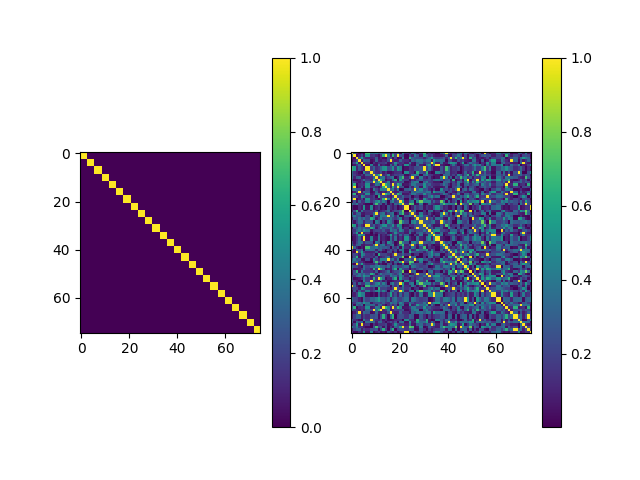
\includegraphics[width=0.9\textwidth]{figures/baseline_sim.png} \label{fig:baseline_sub2} }
    \end{minipage}
    \caption{Here we show a baseline for the node embedding vectors and the final similarity matrix}
    \label{fig:baseline_plot}
\end{figure}

\subsubsection*{Noiseless Dataset}
Here we use no noise to distort it.
This is equivalent to see if Neural Networks can do matrix factorization on a truly low rank matrix.
\begin{figure}[H]
    \centering
    % \includegraphics[width=0.7\textwidth]{figures/noiseless_sim.png}
    \subfloat[Typical embedding and similarity matrix of Noiseless]{ 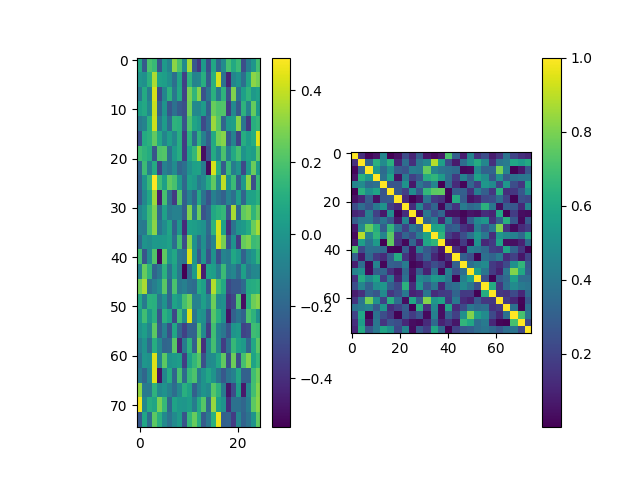
\includegraphics[width=0.45\textwidth]{figures/synth_plot.png} \label{fig:noiseless_sub1} }
    \subfloat[Typical histogram for similarities of noiseless]{ 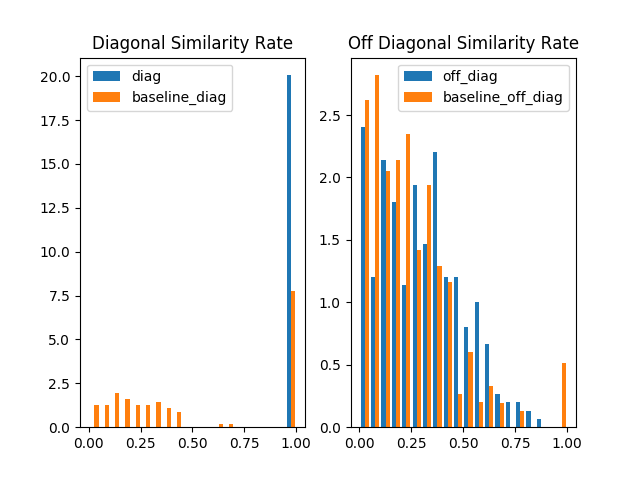
\includegraphics[width=0.45\textwidth]{figures/synth_hist.png} \label{fig:noiseless_sub2} }
    \caption{Here we show a baseline for the node embedding vectors and the final similarity matrix}
    \label{fig:noiseless_plot}
\end{figure}
The numerical scores come out to be:
\begin{table}[H]
    \centering
    \begin{tabular}{|c|c|} \hline
        Trained Same Point Similarity      & 1.00e+00 $\pm$ 8.07e-08  \\ \hline
        Trained Distinct Point Similarity  & 2.81e-01 $\pm$ 1.81e-01  \\ \hline
        Baseline Same Point Similarity     & 5.04e-01 $\pm$ 3.89e-01  \\ \hline
        Baseline Distinct Point Similarity & 2.56e-01 $\pm$ 2.06e-01  \\ \hline
    \end{tabular}
    \caption{Average cross similarity between points, for no noise}
    \label{tab:noiseless_table}
\end{table}

\subsubsection*{Pairwise Matrix Multiplication Noise}
Our noise model for this one $\nu$ is described by, for the block in row $i$, column $j$
\begin{equation*}
    \nu(E)_{ij} = E_i N_{ij} E_j^\top, \quad \quad N_{ij} = \theta I + (1-\theta) \sum_{k=1}^K M_{ij}^k , \quad \quad M_{ij}^{k} \sim {\Pi}(m, m)
\end{equation*}
With the constraint that $N_{ij} = N_{ji}^\top$.
Here $\Pi(m,m)$ denotes the uniform distribution over the $m \times m$ permutation matrices, and $\theta$, and $K$ are parameters.

\paragraph{Parameter Set 1}
Here, $\theta = 0.9$, $K = 1$.
\begin{figure}[H]
    \centering
    % \includegraphics[width=0.7\textwidth]{figures/noiseless_sim.png}
    \subfloat[Typical embedding and similarity matrix of pairwise noise]{ 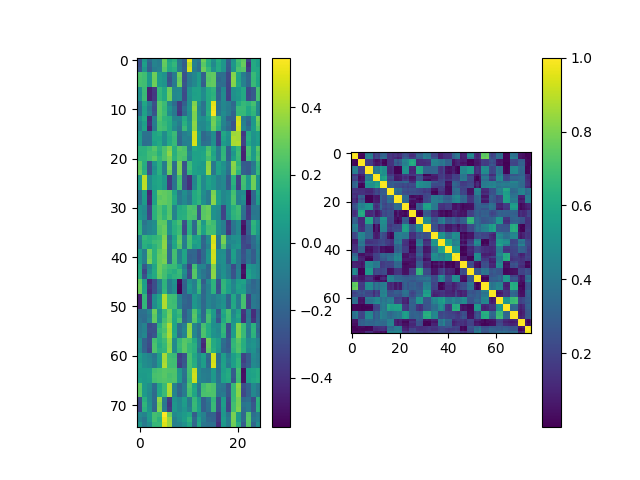
\includegraphics[width=0.45\textwidth]{figures/pairwise_plot.png} \label{fig:pairwise_sub1} }
    \subfloat[Typical histogram for similarities of pairwise noise]{ 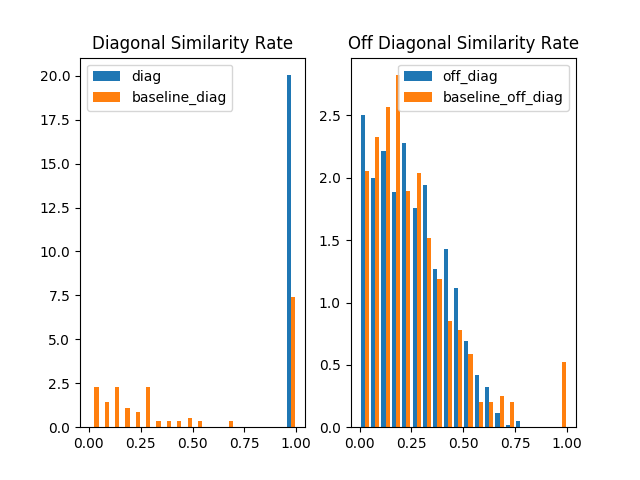
\includegraphics[width=0.45\textwidth]{figures/pairwise_hist.png} \label{fig:pairwise_sub2} }
    \caption{Here we show a baseline for the node embedding vectors and the final similarity matrix}
    \label{fig:pairwise_plot}
\end{figure}
Note the clear separation between diagonal and off diagonal in the histogram. The numerical scores come out to be: 
\begin{table}[H]
    \centering
    \begin{tabular}{|c|c|} \hline
        Trained Same Point Similarity      & 9.97e-01 $\pm$ 4.62e-03  \\ \hline
        Trained Distinct Point Similarity  & 2.86e-01 $\pm$ 1.76e-01  \\ \hline
        Baseline Same Point Similarity     & 5.12e-01 $\pm$ 3.90e-01  \\ \hline
        Baseline Distinct Point Similarity & 2.56e-01 $\pm$ 2.06e-01  \\ \hline
    \end{tabular}
    \caption{Average cross similarity between points, for pairwise noise with $K=1$}
    \label{tab:pairwise_table}
\end{table}

\paragraph{Parameter Set 2}
Here, $\theta = 0.9$, $K = 3$.
\begin{figure}[H]
    \centering
    % \includegraphics[width=0.7\textwidth]{figures/noiseless_sim.png}
    \subfloat[Typical embedding and similarity matrix of pairwise noise]{ 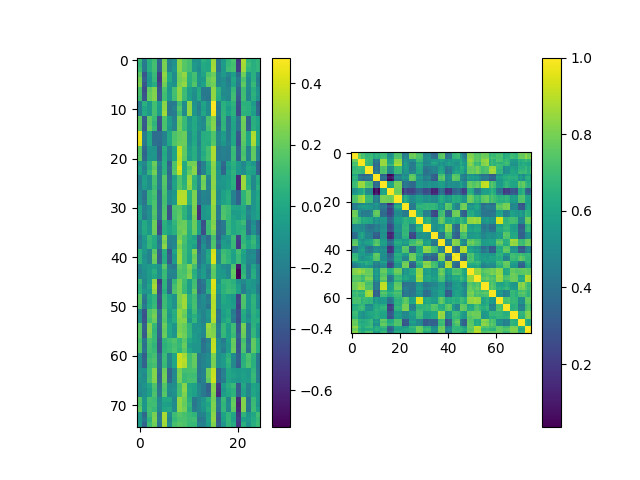
\includegraphics[width=0.45\textwidth]{figures/pairwise3_plot.png} \label{fig:pairwise3_sub1} }
    \subfloat[Typical histogram for similarities of pairwise noise]{ 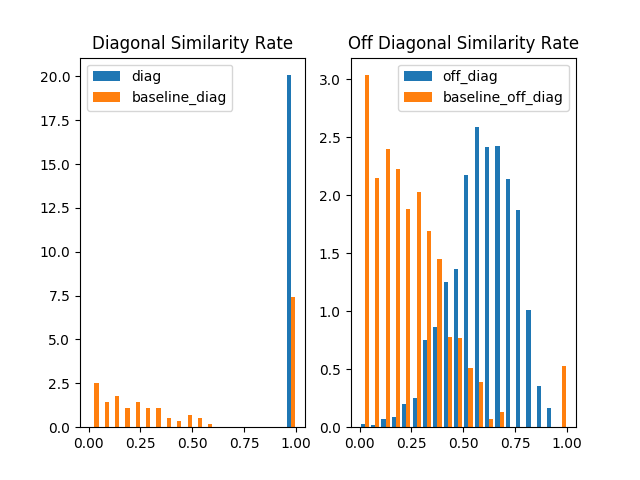
\includegraphics[width=0.45\textwidth]{figures/pairwise3_hist.png} \label{fig:pairwise3_sub2} }
    \caption{Here we show a baseline for the node embedding vectors and the final similarity matrix}
    \label{fig:pairwise3_plot}
\end{figure}
Note that the diagonal and off diagonal entries overlap quite a bit.
The numerical scores come out to be:
\begin{table}[H]
    \centering
    \begin{tabular}{|c|c|} \hline
        Trained Same Point Similarity      & 9.96e-01 $\pm$ 6.24e-03  \\ \hline
        Trained Distinct Point Similarity  & 6.35e-01 $\pm$ 1.42e-01  \\ \hline
    \end{tabular}
    \caption{Average cross similarity between points, for pairwise noise with $K=3$}
    \label{tab:pairwise3_table}
\end{table}

\paragraph{Parameter Set 3}
Here, $\theta = 0.9$, $K = 5$.
\begin{figure}[H]
    \centering
    % \includegraphics[width=0.7\textwidth]{figures/noiseless_sim.png}
    \subfloat[Typical embedding and similarity matrix of pairwise noise]{ 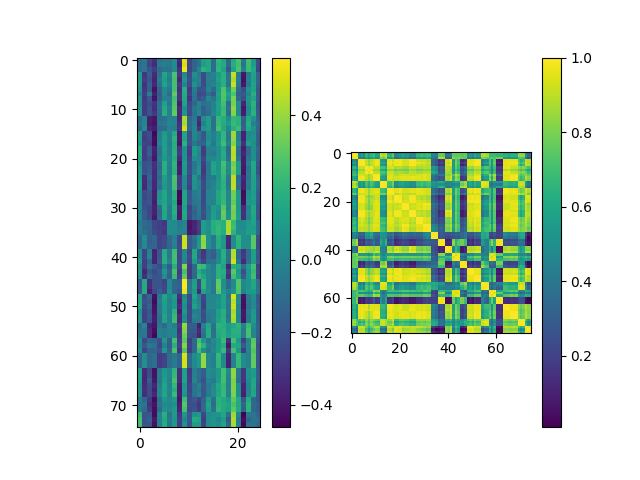
\includegraphics[width=0.45\textwidth]{figures/pairwise5_plot.png} \label{fig:pairwise5_sub1} }
    \subfloat[Typical histogram for similarities of pairwise noise]{ 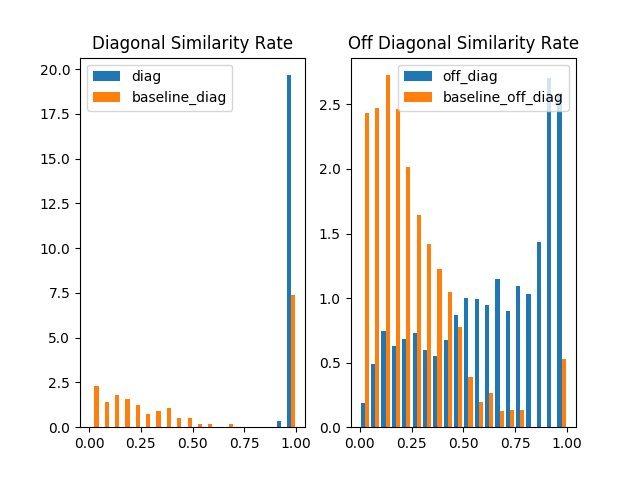
\includegraphics[width=0.45\textwidth]{figures/pairwise5_hist.png} \label{fig:pairwise5_sub2} }
    \caption{Here we show a baseline for the node embedding vectors and the final similarity matrix}
    \label{fig:pairwise5_plot}
\end{figure}
Note that the diagonal and off diagonal entries overlap almost completely.
There is something that goes wrong, and I need to do more investigation before I can determine why.
The numerical scores come out to be:
\begin{table}[H]
    \centering
    \begin{tabular}{|c|c|} \hline
        Trained Same Point Similarity      & 9.90e-01 $\pm$ 2.54e-02  \\ \hline
        Trained Distinct Point Similarity  & 5.82e-01 $\pm$ 3.91e-01  \\ \hline
    \end{tabular}
    \caption{Average cross similarity between points, for pairwise noise with $K=5$}
    \label{tab:pairwise5_table}
\end{table}

\entry{2018}{06}{27}
\subsection*{Larger Dataset Test}
So I was considering that the poor performance might have something to do with overfitting so I decided, since this is synthetic data to generate many more samples in the dataset.
I got the following results for the $K=3$, slightly better than before but within noise.
To put a nail in this coffin, I have been working on generating samples on the fly for training, giving effectively infinite data.
Here are the current results, $\theta = 0.9$, $K = 3$.
\begin{figure}[H]
    \begin{minipage}{.45\linewidth}
        \centering
        \subfloat[Typical embedding and similarity matrix of pairwise noise]{ 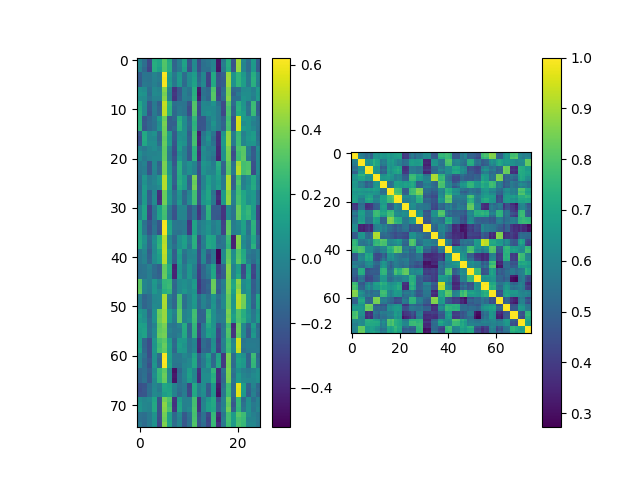
\includegraphics[width=0.9\textwidth]{figures/pairwise3_large_plot.png} \label{fig:pairwise3_large_sub1} }
    \end{minipage}
    \begin{minipage}{.45\linewidth}
        \centering
        \subfloat[Typical histogram for similarities of pairwise noise]{ 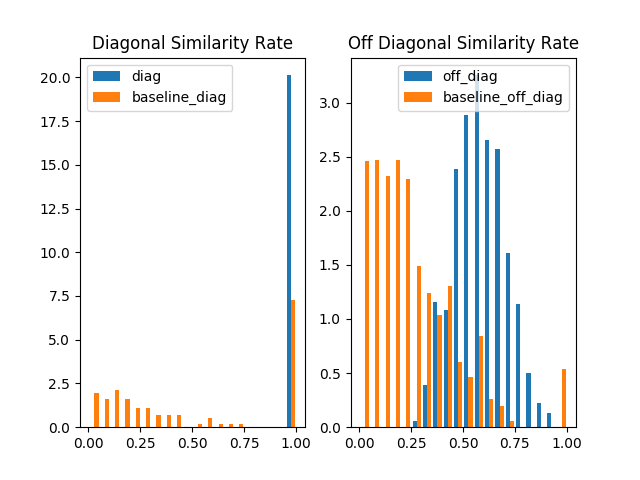
\includegraphics[width=0.9\textwidth]{figures/pairwise3_large_hist.png} \label{fig:pairwise3_large_sub2} }
    \end{minipage}
    \centering
    \subfloat[Numerical results]{
        \begin{tabular}{|c|c|c|c|} \hline
                                       &    Trained Model        &    Previous Model        &    Baseline             \\ \hline
            Same Point Similarity      & 9.97e-01 $\pm$ 4.16e-03 & 9.96e-01 $\pm$ 6.24e-03 & 5.11e-01 $\pm$ 3.91e-01 \\ \hline
            Distinct Point Similarity  & 6.34e-01 $\pm$ 1.29e-01 & 6.35e-01 $\pm$ 1.42e-01 & 2.55e-01 $\pm$ 2.06e-01  \\ \hline
        \end{tabular}
        \label{fig:pairwise3_large_tab1}
    }
    \label{fig:pairwise3_large_plot}
\end{figure}

\entry{2018}{07}{02}
\subsection*{Infinite Dataset Test}
After much debugging to get the data generation during training working, we managed to run some experiments.
Testing with infinite data did seem to improve generalization substantially compared to a simply larger dataset.
So it seems that data is in fact a problem, we will somehow have to address this. 
This is run on the pairwise dataset with $K=3$.
\begin{figure}[H]
    \begin{minipage}{.45\linewidth}
        \centering
        \subfloat[Typical embedding and similarity matrix of pairwise noise]{ 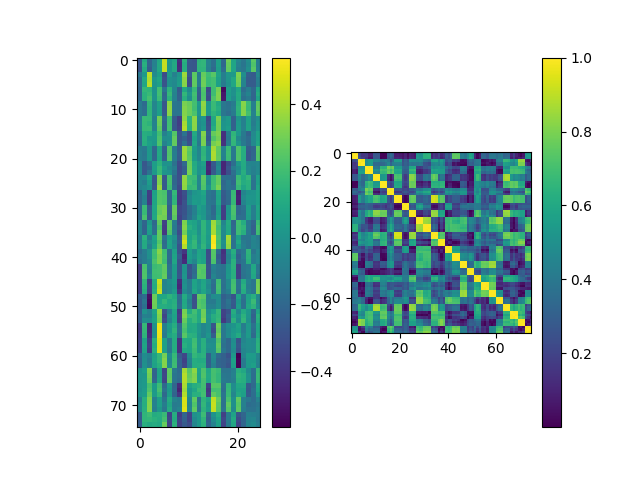
\includegraphics[width=0.9\textwidth]{figures/pairwise3inf_plot.png} \label{fig:pairwise3inf_sub1} }
    \end{minipage}
    \begin{minipage}{.45\linewidth}
        \centering
        \subfloat[Typical histogram for similarities of pairwise noise]{ 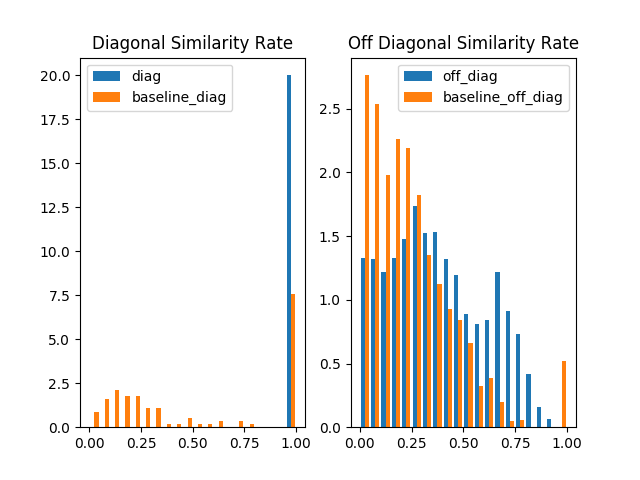
\includegraphics[width=0.9\textwidth]{figures/pairwise3inf_hist.png} \label{fig:pairwise3inf_sub2} }
    \end{minipage}
    \centering
    \subfloat[Numerical results]{
        \begin{tabular}{|c|c|c|c|} \hline
                                       &    Trained Model        &    Previous Model        &    Baseline             \\ \hline
            Same Point Similarity      & 9.96e-01 $\pm$ 5.22e-03 & 9.97e-01 $\pm$ 4.16e-03 & 5.11e-01 $\pm$ 3.91e-01 \\ \hline
            Distinct Point Similarity  & 4.31e-01 $\pm$ 2.15e-01 & 6.34e-01 $\pm$ 1.29e-01 & 2.55e-01 $\pm$ 2.06e-01  \\ \hline
        \end{tabular}
        \label{fig:pairwise3inf_large_tab1}
    }
    \label{fig:pairwise3inf_plot}
\end{figure}
Despite this, the distinction between diagonal and off diagonal entries is not as sharp as I would like.
I need to brainstorm ideas of how to handle that.
There is some work on doing better selection for which edges in the averaging are relevant (e.g. Graph Attention Networks)

\entry{2018}{07}{03}
\subsection*{Infinite Dataset Test}
I ran more experiments with the infinite dataset but with a harder dataset.
This is run on the pairwise dataset with $K=5$.
\begin{figure}[H]
    \begin{minipage}{.45\linewidth}
        \centering
        \subfloat[Typical embedding and similarity matrix of pairwise noise]{ 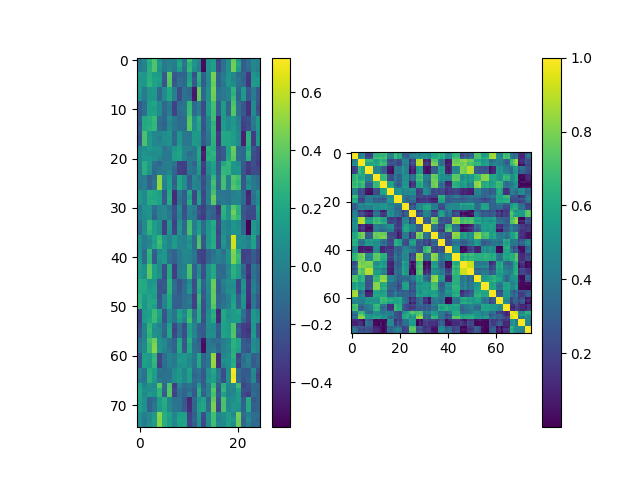
\includegraphics[width=0.9\textwidth]{figures/pairwise5inf_plot.png} \label{fig:pairwise5inf_sub1} }
    \end{minipage}
    \begin{minipage}{.45\linewidth}
        \centering
        \subfloat[For comparison, the non-infinite data trained version]{ 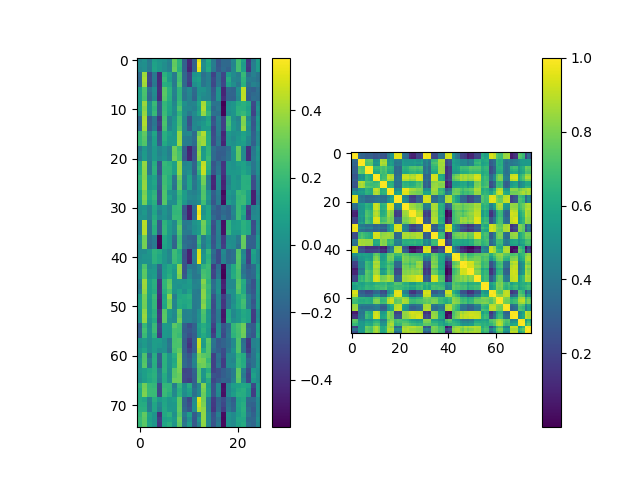
\includegraphics[width=0.9\textwidth]{figures/pairwise5inf_plot_compare.png} \label{fig:pairwise5inf_sub2} }
    \end{minipage}
    \begin{minipage}{.9\linewidth}
        \centering
        \subfloat[Typical histogram for similarities of pairwise noise]{ 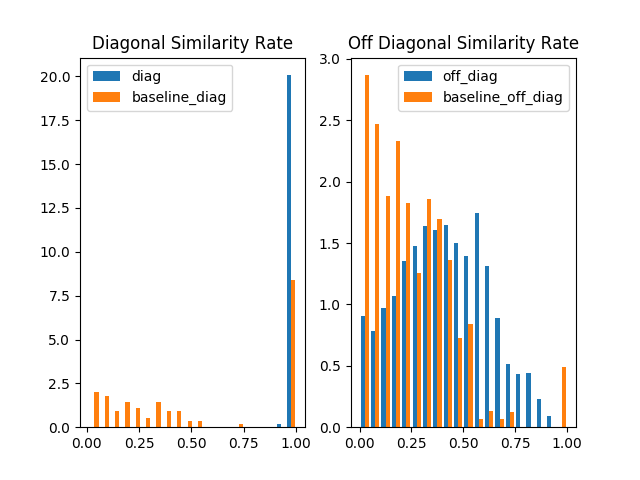
\includegraphics[width=0.5\textwidth]{figures/pairwise5inf_hist.png} \label{fig:pairwise5inf_sub3} }
    \end{minipage}
    \centering
    \subfloat[Numerical results]{
        \begin{tabular}{|c|c|c|c|} \hline
                                       &    Trained Model        &    Previous Model        &    Baseline             \\ \hline
            Same Point Similarity      & 9.97e-01 $\pm$ 3.70e-03 & 9.96e-01 $\pm$ 5.38e-03 & 5.11e-01 $\pm$ 3.91e-01 \\ \hline
            Distinct Point Similarity  & 6.71e-01 $\pm$ 1.55e-01 & 7.13e-01 $\pm$ 1.59e-01 & 2.55e-01 $\pm$ 2.06e-01  \\ \hline
        \end{tabular}
        \label{fig:pairwise5inf_tab1}
    }
    \label{fig:pairwise3inf_large_plot}
\end{figure}
It does OK, but this is still a fairly weak noise model even with the stronger noise.
If the noise got more intense, we would need additional mechanisms to handle it.
Hence the next mechanism.

\subsection*{Graph Attention Network Code Review}
I was looking at the aforementioned Graph Attention Network (GAT) \href{https://arxiv.org/pdf/1710.10903.pdf}{paper} and its \href{https://github.com/PetarV-/GAT}{code}.

\entry{2018}{07}{04}
\subsection*{GAT Implementation details}
After careful looking at the paper and the code for the GAT paper.
After some confusing reading of the code, I figured out the way they are actually implementing it.
It is more naive than I originally thought unfortunately.
Let $E_k$ be the node embedding vectors at the current layer, with adjacency matrix $A$, and weight matrices $T_{k,1}, T_{k,2} \in \mathbb{R}^{n_k \times m_k}$, with $l$ being a point-wise non-linear function, and $s$ being the row-wise-softmax function:
\begin{align*}
f_1 =&\; E_k T_{k,1} \\
f_2 =&\; E_k T_{k,2} \\
Q_k =&\; l(f_1 So \mathbf{1}^\top + \mathbf{1} f_2^\top) \\
E_{k+1} =&\; \sigma \left( s(Q_k + A) E_k W_k \right)
\end{align*}
This has a few problems - This method is really dense.
They have a sparse method but it computes this densely then makes it sparse.
Also if you wanted to enforce the symmetry of the weights on the graph.
. there isn't really a simple way to do that.
Except maybe doing something like using $Q_k' = (Q_k + Q_k^\top)/2$ which doesn't help the whole sparsity problem.
There are some simple ways to make this sparse using for loops but I am uncertain how to do this using TensorFlow... or even PyTorch.
However, as I don't see another way to learn the weights of the edges, this is what I'll be focusing on. 

\subsection*{Leaky ReLU Experiments}
So inspired by the previous paper I thought I would try running experiments with the Leaky ReLU nonlinearity, just to see if it was any different.
As it turns out, unsurprisingly, not too much.

\entry{2018}{07}{05}
\subsection*{Binary Cross Entropy}
Talking with others in the lab (Drew, Oleh) I realized instead of the L2 loss perhaps the Binary Cross Entropy (BCE) Loss would perform better.
Unfortunately this would make it less directly comparable to the optimization methods, but still I think it would worth trying.
First I need to change the datasets to make sure that they don't go over weight 1, which means regeneration of all the datasets.
Next I have to add an addtional loss option for choosing between L2 loss and BCE loss.

\subsection*{TensorFlow Implementation Details}
So my TensorFlow code is OK but it lacks some nice features.
Talking to Drew, it seems Sonnet is the answer, since he showed me some of the features I was missing.
I also need to start using \texttt{SingularMonitoredSession} instead of slim since slim is just... annoying.
So I will need to branch off in git and make a new branch while I get Sonnet working.

\entry{2018}{07}{09}
\subsection*{TensorFlow Implementation Details}
Still working on updating the TensorFlow features to use Sonnet.


\end{document}
